
\begin{figure*}[t]
  \centering
  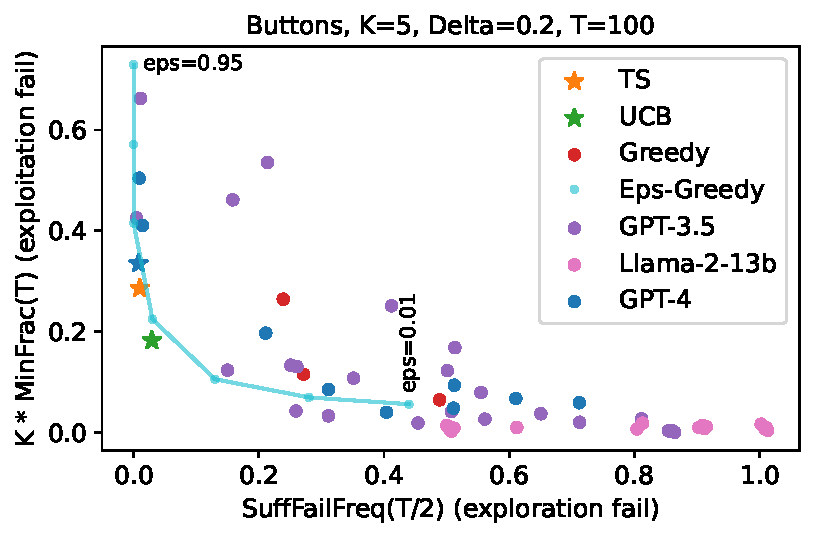
\includegraphics[width=0.6\textwidth]{./figs/fig3.pdf}
  \caption{Scatter plot summarizing all experiments with $T=100$. We plot suffix failures (expressed via $\SuffFailFreq(T/2)$) vs. uniform-like failures (expressed via $K\cdot\MinFrac(T)$).
       Each LLM/configuration pair maps to a dot on this plane (some dots may overlap).
       The \gptfour configuration labeled with a star is BSS$\tC$0, which is the only configuration that succeeds.
       We also plot \EpsGreedy, tracing out the different tradeoffs obtained for different values of $\eps$.}
  \label{fig:scatter}
\end{figure*}

In this section, we present our experimental findings, beginning with a summary in~\Cref{ssec:exp-main}.
In~\Cref{ssec:exp-failures} we investigate failing LLM configurations
in detail, and in~\Cref{ssec:exp-success} we focus on the single
successful LLM configuration our experiments identified.
Finally, in~\Cref{ssec:exp-causes} we attempt to diagnose the underlying causes for exploration failures.



\subsection{Overview}
\label{ssec:exp-main}
We find that all but one of the LLM configurations we consider exhibit exploration failures, not converging to the best
arm with significant probability. This happens either due to
\emph{suffix failures}, where the LLM never selects the best arm after
a small number of initial rounds, or (in a smaller number of configurations) due to \emph{uniform-like
failures}, where the LLM selects all arms at an approximately uniform
rate, failing to eliminate poorly performing arms. The only one
exception is \gptfour with
the BSS$\tC$0 configuration, i.e., with the buttons
scenario, suggestive framing, summarized history, reinforced CoT, and
temperature $0$.



We summarize our key findings in \pref{fig:scatter}
and~\pref{fig:table-gptfour}.
\pref{fig:scatter} summarizes the main set
of experiments (which we recall consider the \hard MAB instance), visualizing each LLM
configuration with a single point on a scatter plot where the
axes correspond to two \emph{surrogate statistics},
$\SuffFailFreq$ and $\MinFrac$, which represent the
strength of the two failure modes ($\SuffFailFreq$ measures
suffix failures, and $K\cdot\MinFrac$ measures uniform-like failures); these statistics are described in detail in the sequel. \pref{fig:table-gptfour}
displays $\SuffFailFreq$, $\MinFrac$, $\GreedyFrac$ (which measures how similar a method is to \greedy), and additional summary statistics for each of the \gptfour configurations in
the main set of experiments. These statistics reveal that all of the LLM configurations, except for
\gptfour-BSS$\tC$0 (the blue star
in~\pref{fig:scatter}), behave fundamentally differently from the
baseline algorithms \ucb and \ts, and we find that these
differences result in a large, persistent drop in performance.
Conversely, we find that \gptfour-BSS$\tC$0 successfully explores and (as a result) converges to the best arm.


\begin{figure*}
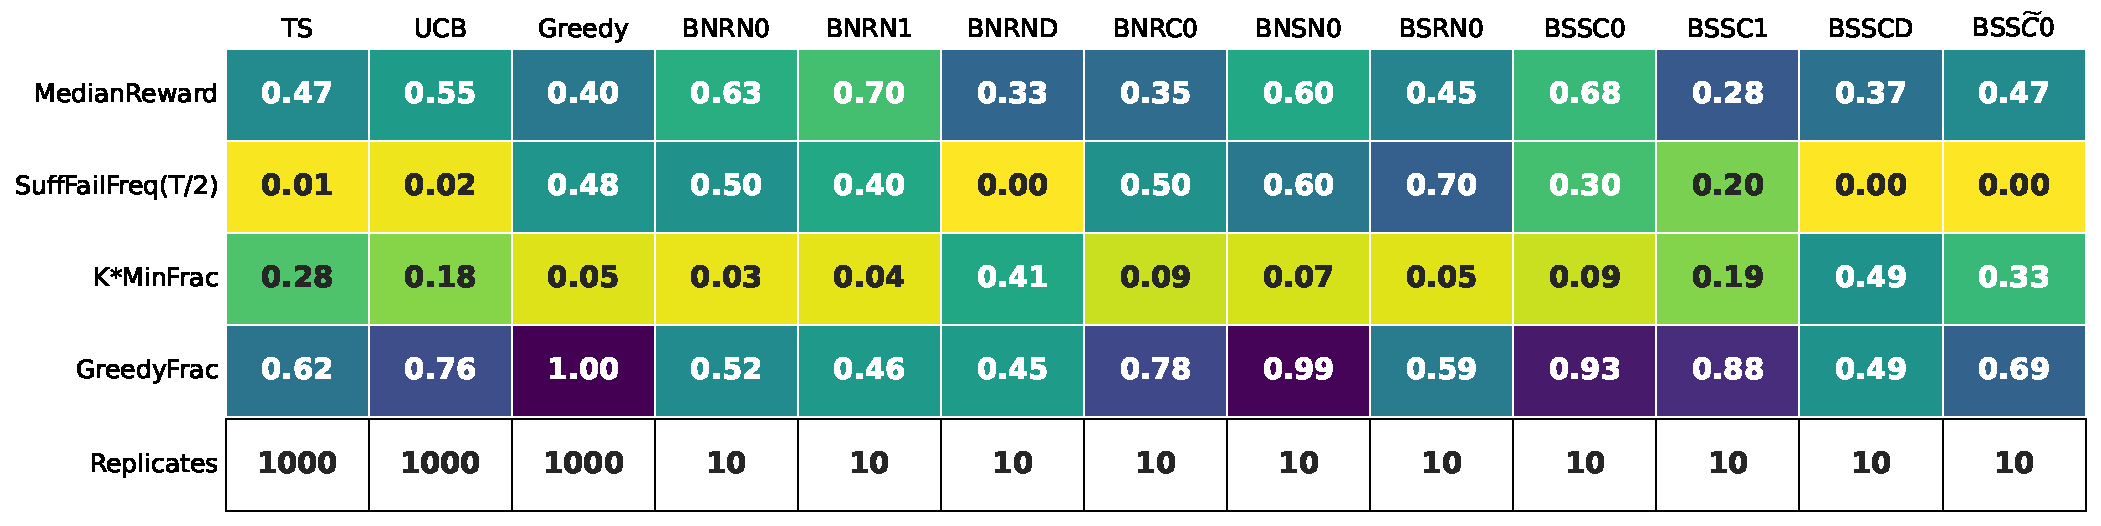
\includegraphics[width=\textwidth]{./figs/fig10.pdf}
\caption{ \gptfour for $T=100$: a per-configuration \textbf{summary
    table} on the \hard MAB instance.  
  Only
  three \gptfour configurations do not exhibit suffix failures; two of
  these (BNRND and BSSCD) exhibit uniform-like failures. The final
  configuration (BSS$\tC$0) succeeds.  }
\label{fig:table-gptfour}
\end{figure*}





\begin{figure*}[t]
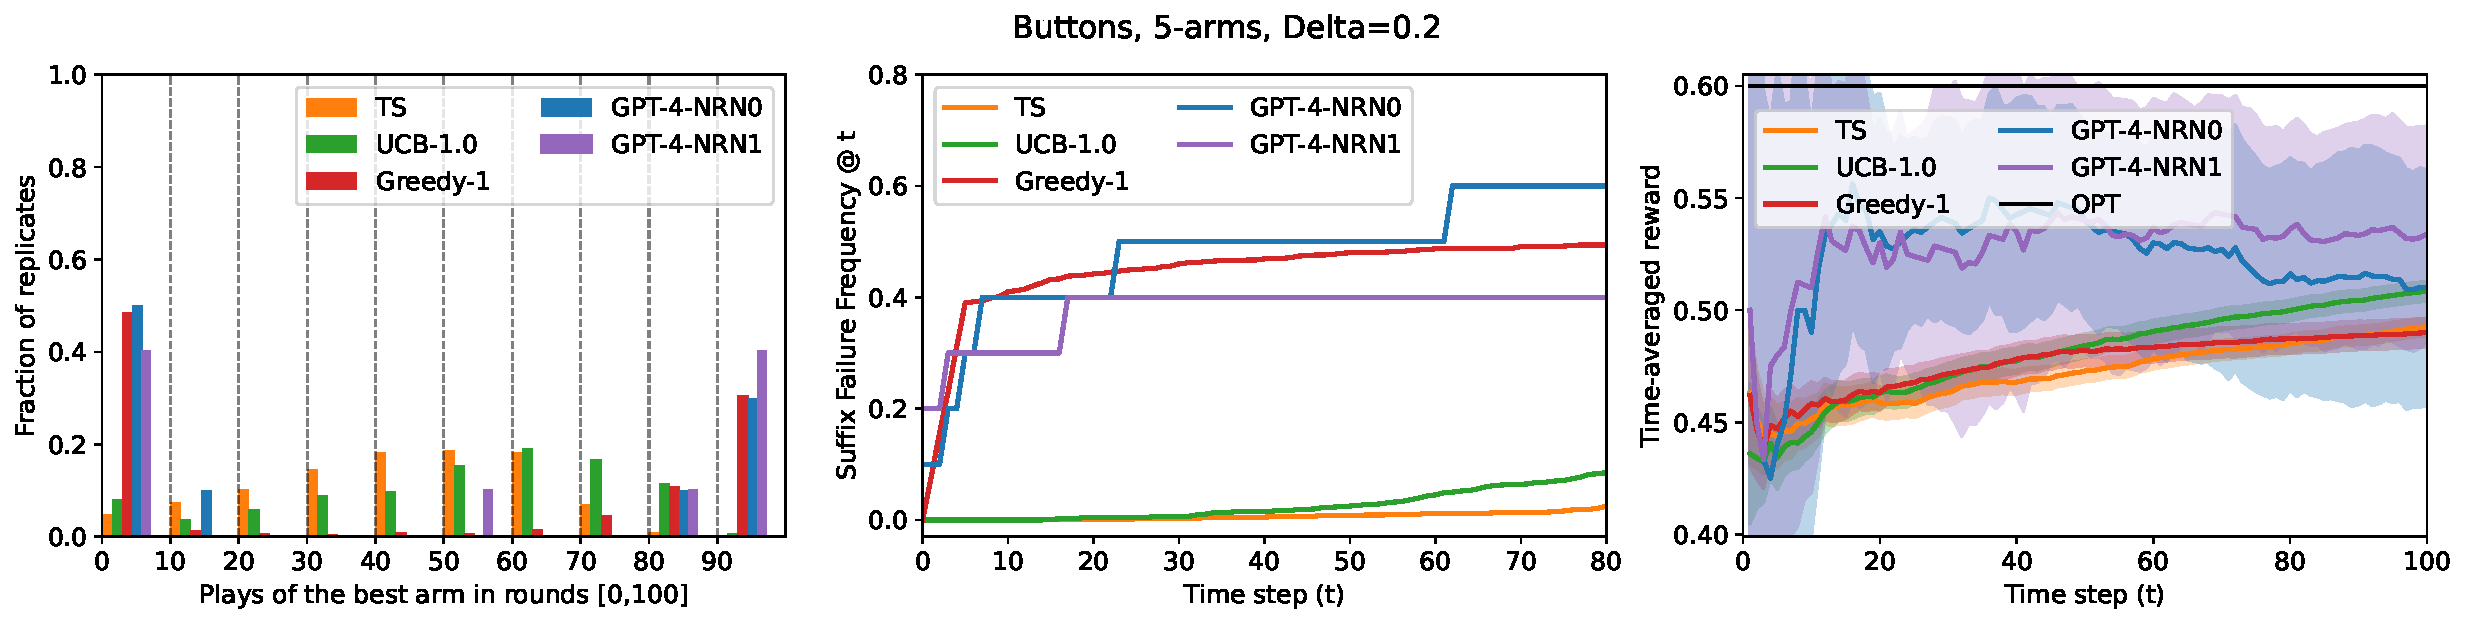
\includegraphics[width=\textwidth]{./figs/fig4.pdf}
\caption{Detailed view of bimodal behavior and suffix failures for \gptfour with $T=100$. Configurations visualized are the basic configuration (BNRN0) and the same configuration but with temperature $1$ (BNRN1). Visualizations are the same as in~\pref{fig:long}.}
\label{fig:main-ex-a}
\end{figure*}

\subsection{Identifying failures}
\label{ssec:exp-failures}


We now give a precise overview of the exploration failures illustrated in
\cref{fig:scatter} and \cref{fig:table-gptfour}, and provide
additional results and figures that illustrate failure in greater detail. We focus 
on \gptfour, as
we find that \gptthree and \llama perform worse (and often \emph{much}
worse) in all experiments; detailed results for \gptthree and \llama
are included in~\pref{app:summary-figures} for completeness. We begin
with detailed background on the surrogate statistics, $\SuffFailFreq$
and $\MinFrac$, used to quantify failures
in~\cref{fig:scatter,fig:table-gptfour} and beyond, providing evidence that exploration
failure---as quantified by these statistics---results in a persistent drop in performance.

\xhdr{Suffix failures.}
Most of the LLM configurations we consider exhibit highly
\emph{bimodal} behavior, whereby a large fraction of the replicates
choose the best arm very rarely, and a few
replicates converge to the best arm extremely quickly. Consistent with
this bimodal behavior, we observe a large incidence of \emph{suffix
  failures}, where the best arm is not selected even once after a
small number initial of rounds (i.e., in some ``time suffix"). Suffix failures are suggestive of a long-term failure to explore which cannot be improved by running the algorithm for longer, because, without playing the optimal arm, one cannot acquire information to learn that it is indeed optimal. Such behaviors
are qualitatively similar to those of \greedy
and qualitatively very different from those of \ucb and Thompson Sampling.

Our surrogate statistic for measuring suffix failures is defined as
follows: For an experiment replicate $R$ and round $t$, let
$\SuffFail(t,R)$ be a binary variable that is $1$ if the best arm is
never chosen in rounds $[t,T]$. Then let $\SuffFailFreq(t) :=
\text{mean}(\cbr{\SuffFail(t,R):\, \text{replicates $R$}})$. Suffix failures manifest in most of our experiments at $T=100$.
In the scatter plot in~\pref{fig:scatter}, the X-axis plots $\SuffFailFreq(T/2)$ for each
LLM configuration, and we find that all but five configurations have
$\SuffFailFreq(T/2) \geq 15\%$. Recalling the definition of suffix
failures, this means that $\geq15\%$ of the time, these configurations do
not pull the best arm \emph{even once} in the last half of the rounds.

A more detailed view of suffix failures and bimodal behavior can be
obtained by focusing on individual LLM configurations. We visualize
this for the basic configuration (\gptfour-BNRN0) in~\pref{fig:long} (top) for $T=500$, and
in~\pref{fig:main-ex-a} for \gptfour (BNRN0 and BNRN1) at $T=100$.
In these detailed views, the middle panels plot $\SuffFailFreq(t)$ at
each time $t$ for the given LLM configurations, as well as \ucb, \ts, and \greedy. We find that these LLM configurations have much higher suffix failure rates than both \ucb and \ts.
 Bimodal behavior
is visualized in the left panel of each plot, where for each
configuration, a large fraction of replicates rarely pulls the best
arm, while the remaining fraction almost always pulls the best arm.
Because of this bimodal behavior (particularly because a constant
fraction of replicates by chance
almost always pull the best arm), suffix failures are not fully
reflected in the total reward plots in the right panels of \cref{fig:main-ex-a}, since the time horizon $T=100$ is not large enough.  However, as mentioned,
suffix failures are suggestive of an irrecoverable failure to explore
which leads to stark differences in reward for larger $T$.  This
is precisely what we find at $T=500$ in~\pref{fig:long},
which suggests that suffix failures indeed lead to poor long-term
performance.


\xhdr{Uniform-like failures.}
Returning to the left panel of~\pref{fig:scatter}, we see that three \gptfour configurations avoid suffix failures.
Two of these configurations exhibit a different type of failure,
where the LLM selects arms in roughly equal
proportions for the entirety of the $T$ rounds and fails to exploit the acquired information to focus on the better arms.
We call this a \emph{uniform-like failure}.

Our surrogate statistic for measuring such failures is defined as follows: For a particular experiment replicate $R$ and round $t$, let $f_a(t,R)$ be the fraction of rounds in $[1,t]$ in which a given arm $a$ is chosen, 
    $\MinFrac(t,R) := \min_a f_a(t,R)$, and
    $\MinFrac(t):= \text{mean}(\cbr{\MinFrac(t,R):\, \text{replicates $R$}}) $.
Since $\MinFrac(t) \leq 1/K, \; \forall t \in [T]$, we always plot
    $K\cdot \MinFrac(t)$,
so as to rescale the range to $[0,1]$.
Larger $\MinFrac(t)$  corresponds to a more uniform selection of arms
at time $t$. When an LLM's $\MinFrac(t)$ does not decrease over time
and stays substantively larger than that of the baselines (especially
as $t$ approaches the time horizon $T$), we take it as an indication of a uniform-like failure.


\begin{figure*}[t]
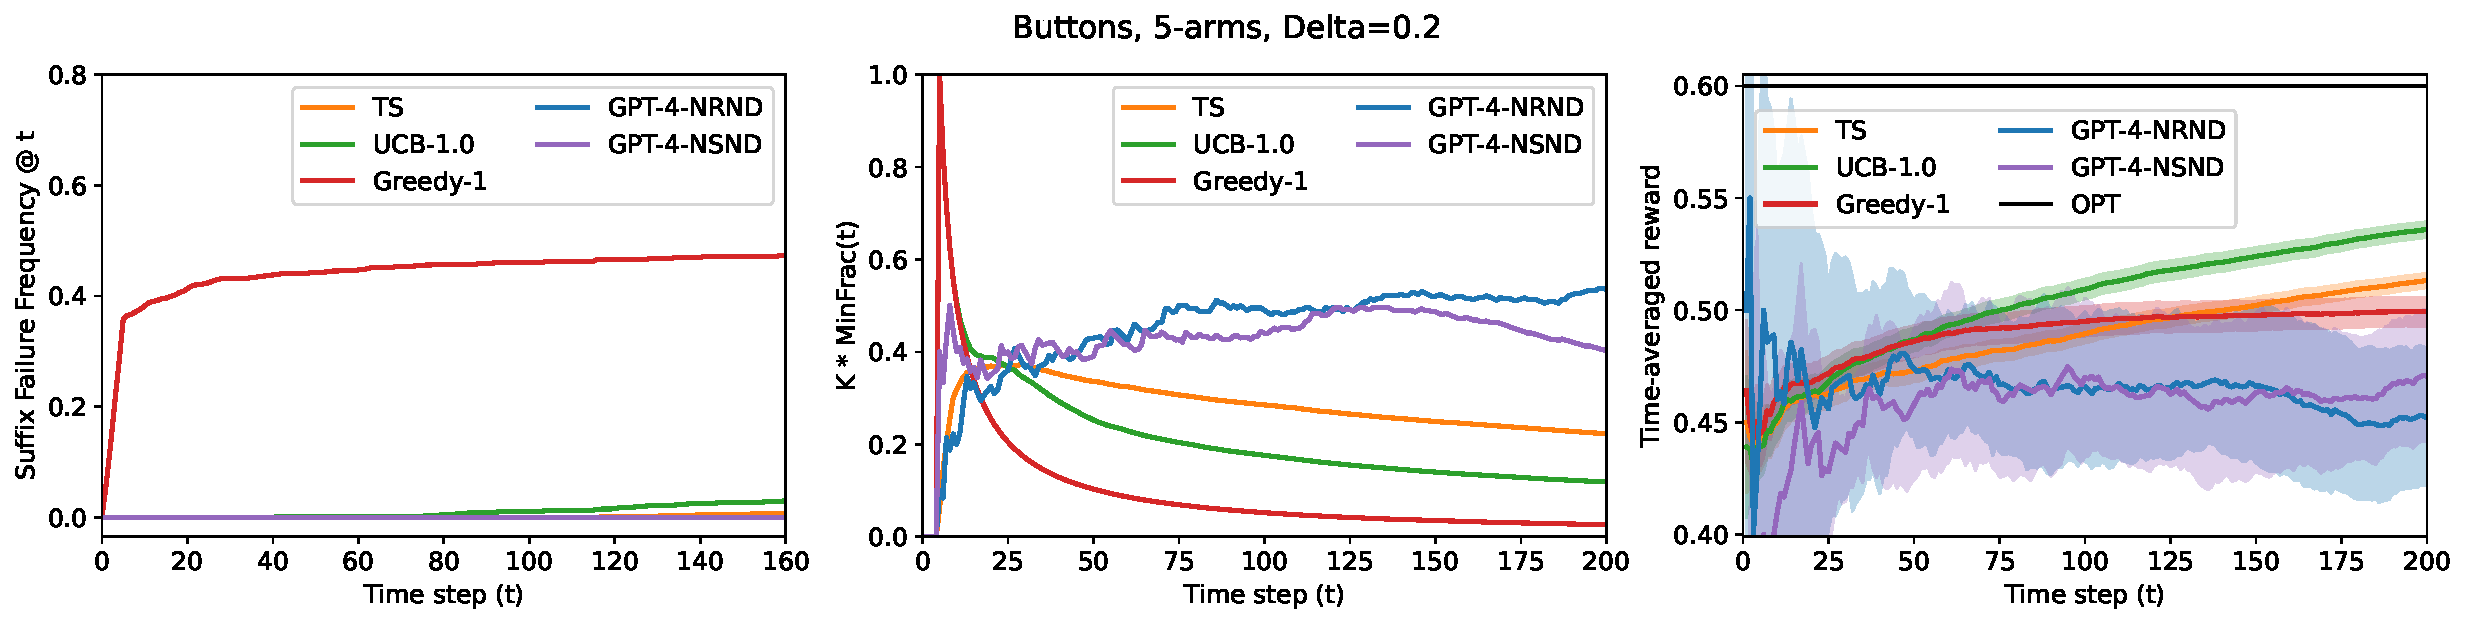
\includegraphics[width=\textwidth]{./figs/fig5.pdf}
\caption{Detailed view of uniform-like failures for \gptfour (the BNRND and BNSND configurations) with $T=200$. Visualizations are: (Left) suffix failure frequency, (Center) $K\cdot\MinFrac(t)$ as a function of $t$ and (Right) cumulative time-averaged rewards.
  These configurations exhibit uniform-like failures but not suffix failures, and uniform-like failures are detrimental to long-term rewards.}
\label{fig:main-ex-b}
\end{figure*}

The Y-axis of~\pref{fig:scatter} records $K\cdot\MinFrac(T)$ for each
configuration, where we see that of the three \gptfour configurations
that avoid suffix failures, two configurations have very high $\MinFrac(T)$ relative to
\ucb and \ts (the third configuration is \gptfour-BSS$\tC$0, which is successful).  These two configurations are \gptfour-BNRND and
\gptfour-BSSCD, both of which use the \emph{distributional} output format.
We provide a more detailed view of \gptfour-BNRND (as well as 
\gptfour-BNSND, which also exhibits uniform-like failures, but only differs from \gptfour-BNRND in the use of summarized history)
in~\pref{fig:main-ex-b}, which considers a longer horizon and more
replicates ($T=200$ and $N=20$).  The middle panel reveals that
$K\cdot\MinFrac(t)$ does not decrease over time for these LLM configurations, while it
does for the baselines.  This behavior results in no suffix failures,
but leads to much lower reward than the baselines.  In particular, we obtain a clear separation in
total reward, showing that uniform-like failures indeed result in poor
long-term performance.



\xhdr{Generality of the failures.}
To summarize, \pref{fig:scatter} shows that all LLM configurations except \gptfour-BSS$\tC$0 exhibit either a suffix failure or a uniform failure for the \hard MAB instance and the buttons scenario.
Scatter plots for the other three experiments (\ie the advertisements scenario and/or the \easy MAB instance) are qualitatively similar and are deferred to~\pref{app:summary-figures}.



\newcommand{\AveRew}{\Phi}

The same data, but with attributions to specific LLM configurations,
are presented for \emph{all} \gptfour configurations in \pref{fig:table-gptfour}; analogous
tables for other LLMs and experimental settings are given in~\pref{app:summary-figures}. %
As it is not instructive to present detailed plots such as
\pref{fig:main-ex-a} for every LLM configuration,
\cref{fig:table-gptfour} summarizes the performance of each configuration with just a few statistics. We include:
\begin{itemize}
\setlength{\itemsep}{0pt}
\item $\SuffFailFreq(T/2)$ and $\MinFrac(T)$, defined above.
\item $\MedRew$: the rescaled median (over replicates) of the time-averaged total reward.%
\footnote{More precisely, let $\AveRew(R)$ be the time-averaged total reward for a given replicate $R$. Then
    $\E\sbr{\AveRew(R)}$ ranges in the interval $[\nicefrac12-\Delta/2,\, \nicefrac12+\Delta/2 ]$.
We rescale $\AveRew(R)$, by translating and multiplying, so that $\E\sbr{\AveRew(R)}$ ranges in $[0,1]$.}
\item $\GreedyFrac$: the fraction of \emph{greedy rounds}, averaged over the replicates. A greedy round is one in which an arm with a largest average reward is selected. This is one way to quantify the extent to which a configuration behaves like \greedy.
\end{itemize}

\begin{figure*}
\centering
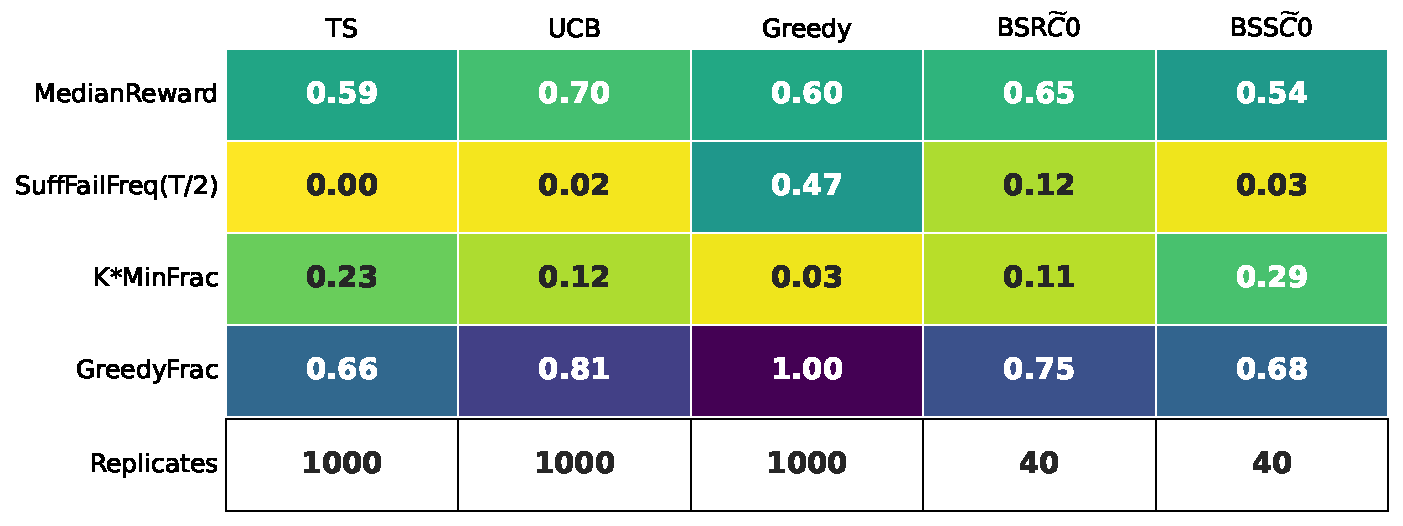
\includegraphics[width=0.8\textwidth]{./figs/fig6.pdf}
\caption{Summary statistics of two \gptfour configurations with reinforced CoT
  (BSR$\tC$0 and BSS$\tC$0) when run on the \hard MAB
  instance with $T=200$ for $N=40$ replicates. BSR$\tC$0 exhibits suffix
  failures. BSS$\tC$0 exhibits neither suffix failures nor uniform-like
  failures and has reasonable reward, so we declare it to be successful.  }
\label{fig:table_reinforced_cot}
\end{figure*}

We now summarize
further findings from the scatter plots (\Cref{fig:scatter,fig:main-scatter-all}) and
the summary tables (\Cref{fig:table-gptfour-all,fig:gpt35_table_buttons_hard,fig:gpt35_table_adverts_hard,fig:gpt35_table_buttons_easy,fig:gpt35_table_adverts_easy,fig:llama_table_buttons,fig:llama_table_adverts}). First, \gptfour performs much better than
\gptthree, and \llama performs much worse (in particular, the suffix
failure frequency for \llama ranges from that of \greedy to much
larger). Second, we observe that all LLMs are sensitive to small changes in
the prompt design. However, the different modifications we consider
appear to interact with each other, and it is difficult to identify
which individual modifications improve performance and which degrade it.

\subsection{Investigating successes}
\label{ssec:exp-success}
On the \hard MAB instance, the only configuration in our experiments
that avoids both suffix failures and uniform-like failures is \gptfour
with the BSS$\tC$0 prompt design. As can be seen
from~\pref{fig:table-gptfour}, at $T=100$, this configuration has no
suffix failures, the $K\cdot\MinFrac$ value is only slightly larger than
\ts, and the reward is comparable to \ts. These statistics suggest
that this configuration succeeds, and in this section we present
further evidence supporting this claim.

\begin{figure*}[t]
  \centering
  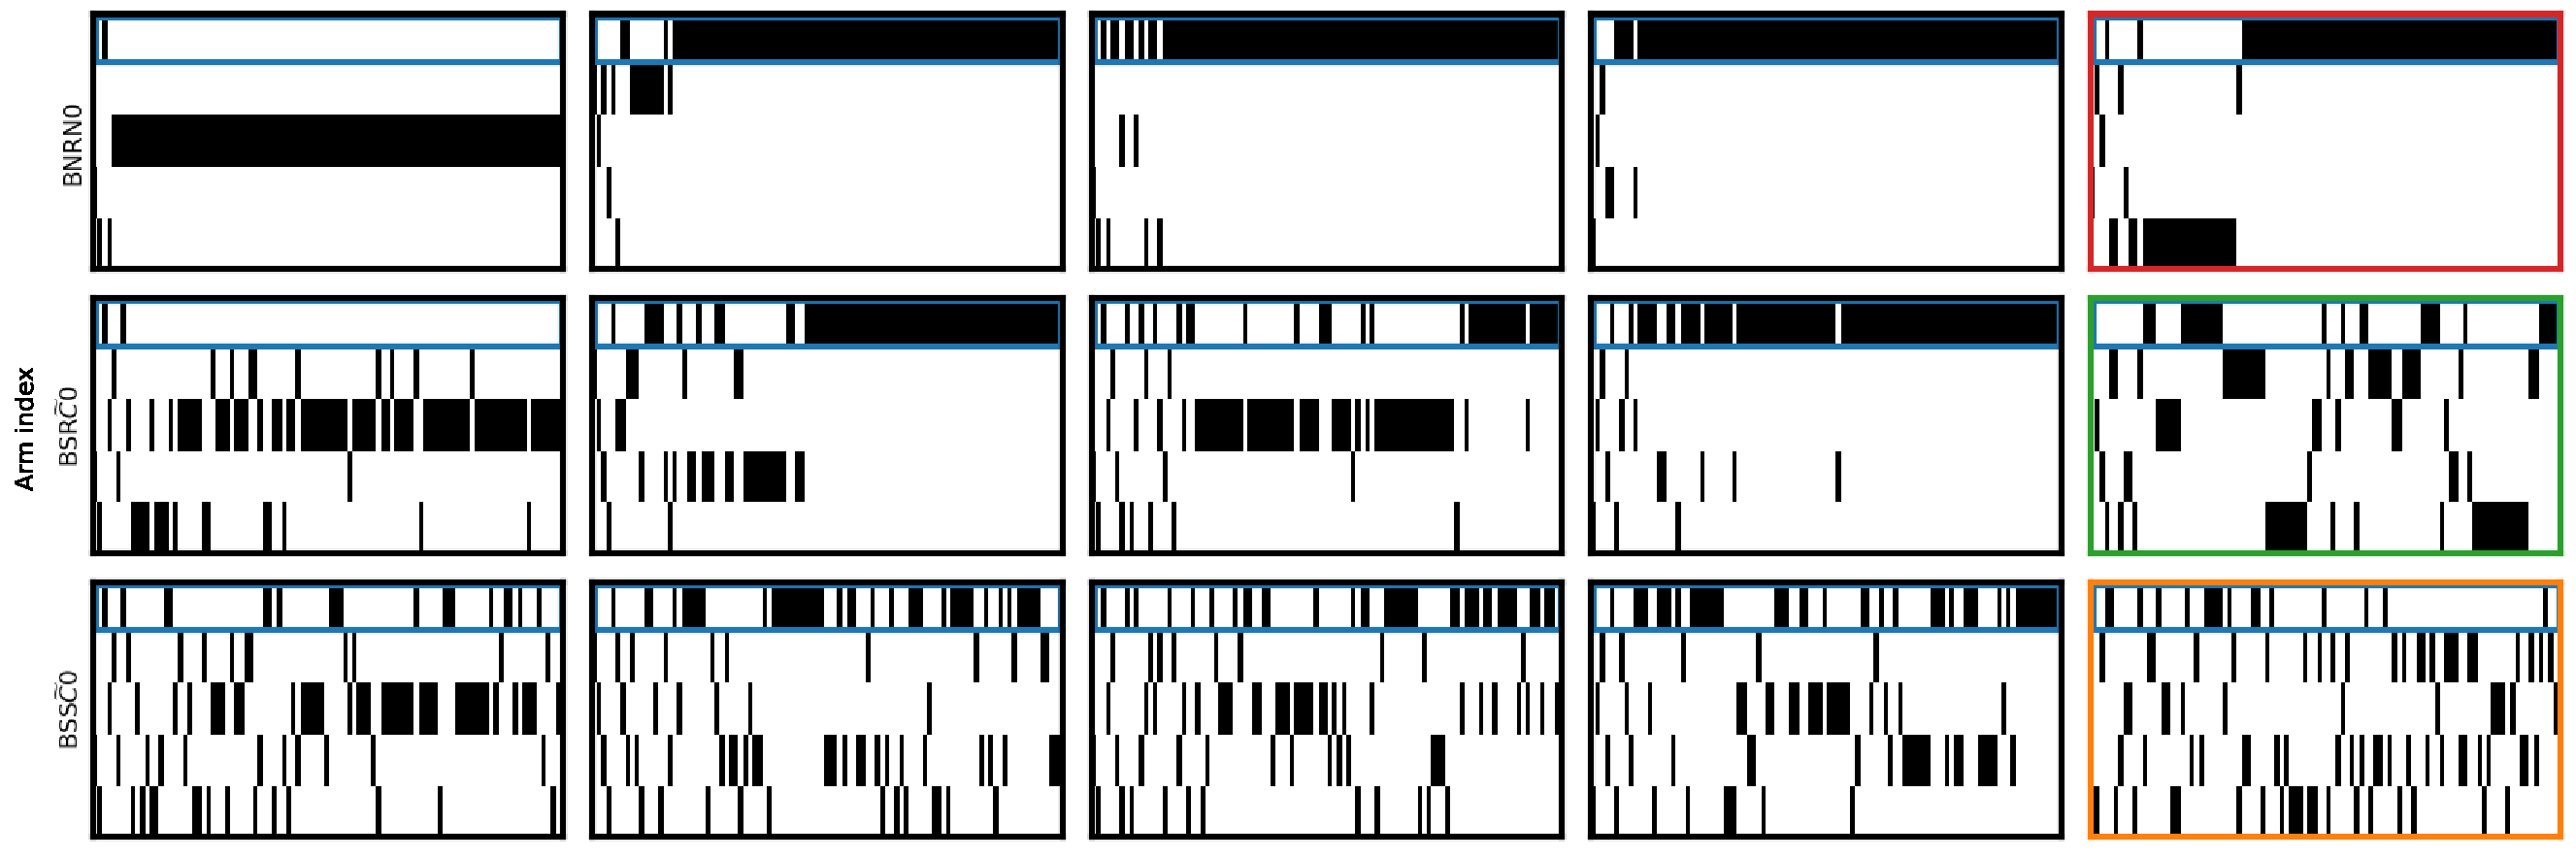
\includegraphics[width=\textwidth]{./figs/fig7.pdf}
  \caption{Traces of the arm chosen at each time step for (a) $4$ of
    the replicates of the basic configuration (\gptfour-BNRN0) (left
    four cells in top row), (b) $4$ of the replicates of
    \gptfour-BSR$\tC$0 (left four cells of the middle row), (c) $4$ of
    the replicates of \gptfour-BSS$\tC$0 (left four cells of the
    bottom row), as well as one replicate of \greedy (red border),
    \ucb (green border) and \ts (orange border).  For each of the
    $T=100$ time steps (X-axis) we indicate which of the five arms was
    chosen (Y-axis). The best arm is the top row of each plot,
    highlighted with blue boxes.}
  \label{fig:traces}
\end{figure*}

\begin{figure*}[t]
  \centering
  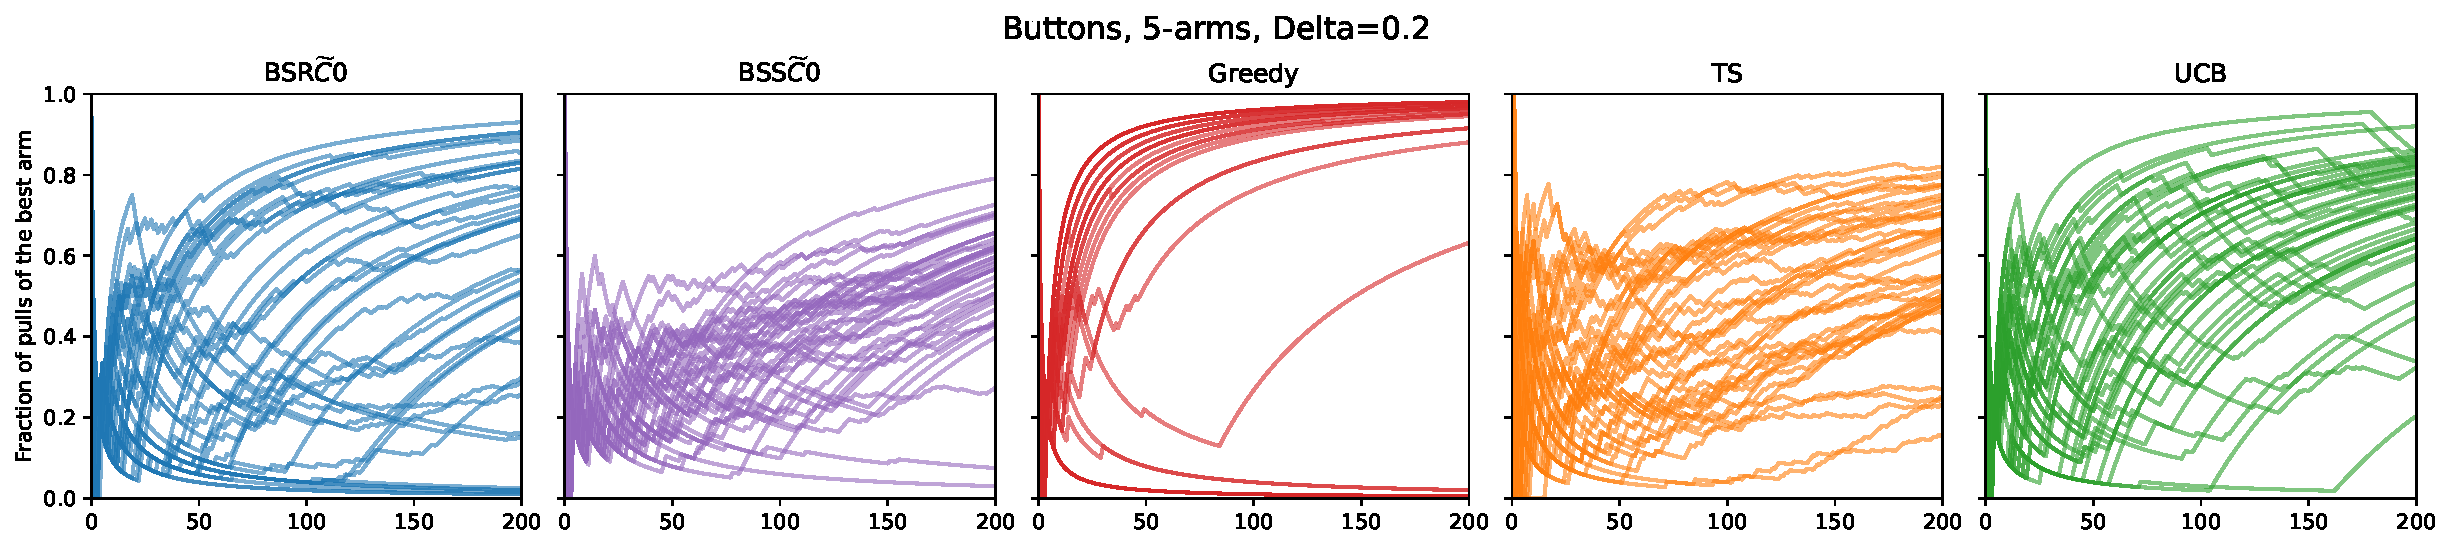
\includegraphics[width=\textwidth]{./figs/fig8.pdf}
  \vspace{-0.75cm}
  \caption{Visualization of the per-replicate behavior of two \gptfour
    configurations with reinforced-CoT and the baselines. For each algorithm,
    replicate and time step $t$, we plot the fraction of rounds in
    $[0,t]$ where the optimal arm was pulled.}
  \label{fig:per-rep}
\end{figure*}

To do so, we run \gptfour-BSS$\tC$0 on the \hard MAB
instance with $T=200$ and $N=40$ to obtain more statistically
meaningful results. We also consider
\gptfour-BSR$\tC$0, which swaps summarized history
for raw history, as an ablation.~\pref{fig:table_reinforced_cot}
provides a summary of the results from this experiment,
while~\pref{fig:long}(b) provides a detailed view of the
BSS$\tC$0 configuration.  The figures reveal that
BSS$\tC$0 continues to avoid suffix failures and
performs relatively well in terms of reward for larger $T$. On the other hand, we see
that BSR$\tC$0 exhibits a non-trivial fraction of
suffix failures, demonstrating that this ablation results in
fundamentally different behavior.

We also provide two additional visualizations that provide some
qualitative evidence toward the success of BSS$\tC$0,
as well as the failure of other configurations. These are presented
in~\pref{fig:traces} and~\pref{fig:per-rep}.  In~\pref{fig:traces} we
visualize the arm chosen at each time step for various replicates of
several different methods (LLMs and baselines). Specifically, \cref{fig:traces} shows
four replicates for the basic configuration (BNRN0) and the
two configurations with reinforced CoT (BSR$\tC$0 and
BSS$\tC$0), as well as one replicate of each of the
baseline algorithms. We see that the basic configuration BNRN0 tends to commit to a
single arm for several rounds, a behavior that is similar to that of
\greedy and very different from both \ucb and \ts.
BSR$\tC$0 also commits for long periods, but to a lesser extent than
the basic configuration.  In contrast, BSS$\tC$0
switches arms much more frequently, and qualitatively appears much more
similar to \ts.

In~\pref{fig:per-rep}, we plot the fraction of rounds in $[0,t]$ where
the optimal arm was pulled as a function of $t$ for individual
replicates.  BSR$\tC$0 is visually similar to
\ucb, except that a non-trivial fraction of runs exhibit suffix failures (the curves that converge to
$0$ on the plot). Meanwhile, BSS$\tC$0 is visually 
similar to \ts, with almost all replicates slowly converging to $1$.
These visualizations, along with the summary statistics,
suggest that BSS$\tC$0 behaves most similarly to
\ts, which further suggests it will successfully converge to the
optimal arm given a long enough time horizon.







\subsection{Root causes}
\label{ssec:exp-causes}
\begin{wrapfigure}{r}{0.45\textwidth}
  \vspace{-0.5cm}
    \centering
    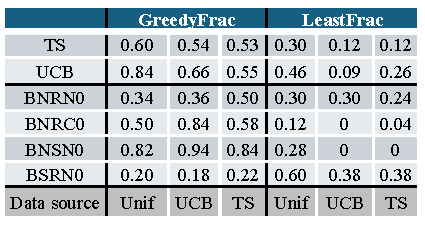
\includegraphics[width=0.45\textwidth]{puzzles.pdf}
    \caption{Per-round decisions with some \gptthree configurations.
    $T=100$, histories of length $t=30$, \hard MAB instance.}
    \label{fig:puzzles}
\end{wrapfigure}

Our experimental findings above shed light on how LLM-based decision
making agents
behave, but it is also worthwhile to understand \emph{why} they behave
the way they do (and particularly, why they fail).  This question is
rather challenging to answer decisively, but two natural hypotheses
are that the configurations we consider (outside of \gptfour-BSS$\tC$0) are either a) too greedy, or b) too uniform-like. In
this section, we describe how our experiments offer some insight into
this hypotheses.

First, focusing on \gptfour, our experiments reveal qualitatively
different behavior between the \easy and \hard instances (\Cref{fig:table-gptfour-all}(a) and \Cref{fig:table-gptfour-all}(c)).
Indeed, the \easy instance appears to be \emph{much} easier; most
\gptfour configurations avoid suffix failures and accrue large rewards
on this instance, and the $\GreedyFrac$ statistic offers a potential explanation as to why.
On the \easy instance, most \gptfour configurations have very high $\GreedyFrac$ values, so they behave similarly to \greedy, which performs quite well (even though \greedy provably fails with small constant probability and, empirically, has many suffix failures on this instance).\footnote{Indeed, in~\pref{fig:table-gptfour-all}(c) we see that most \gptfour configurations have very high $\GreedyFrac$ but no suffix failures. Apparently, even a very small amount of exploration suffices for easy instances (and makes a big difference, relative to \greedy). However, this should not be construed as evidence for the more general and robust exploratory behavior necessary for harder bandit instances.}
A plausible hypothesis from this is that \gptfour performs quite well in low-noise settings, which is precisely when \greedy also performs well.\loose

A stronger hypothesis would be that most \gptfour configurations (except perhaps those using reinforced CoT) behave like \greedy on \emph{all} instances, but this hypothesis is invalidated by the $\GreedyFrac$ statistics for our experiments on the \hard instance.
On the \hard instance, it seems that most \gptfour configurations are
doing something non-trivial (albeit flawed); their behavior is neither
completely \greedy-like nor like uniform-at-random.


Toward a more fine-grained understanding, we ran a collection of small-scale secondary experiments focusing on the \emph{per-round decisions} of LLM-agents.
The experiments focus on a single round $t$ in a bandit problem. Each
experiment considers a particular ``data source" (a distribution of
bandit histories), samples $N=50$ bandit histories of length $t$ from this
distribution, and presents them to the agents (the LLMs and the
baselines) and asks them to output an arm or distribution over
  arms. We track two statistics for each agent: $\GreedyFrac$ and
$\LeastFrac$, the fraction of replicates in which the agent chose,
resp., an empirically best arm so far and a least-chosen arm so
far. We vary the data source, i.e., the algorithm which generates the
history. In particular, we consider histories generated by sampling
uniformly at random (\texttt{Unif}) and by running our baselines \ucb
and \ts for $t$ rounds.\loose 

Results are summarized in \cref{fig:puzzles}.  Unfortunately, we
find that per-round performance of both the LLMs and the baselines is very
sensitive to the particular data source. For example, the $\MinFrac$
statistic of \ucb can vary from as high as 0.46 on histories generated
uniformly at random to as low as 0.09 on histories generated by \ucb
itself. It seems plausible to conclude the BNSN0 is too greedy while
BSRN0 is too uniform, but the statistics for the other two LLM
configurations (BNRN0 and BNRC0)---both of which fail in our
longitudinal experiments---fall within the reasonable range provided
by the baselines.  Thus, we find that it is challenging to assess whether
LLM agents are too greedy or too uniform-like based on per-round
decisions, even though these agents behave rather differently from the
baselines in the longitudinal experiments.













